% Options for packages loaded elsewhere
\PassOptionsToPackage{unicode}{hyperref}
\PassOptionsToPackage{hyphens}{url}
\PassOptionsToPackage{dvipsnames,svgnames,x11names}{xcolor}
%
\documentclass[
  a4paper,
  DIV=11,
  numbers=noendperiod]{scrartcl}

\usepackage{amsmath,amssymb}
\usepackage{iftex}
\ifPDFTeX
  \usepackage[T1]{fontenc}
  \usepackage[utf8]{inputenc}
  \usepackage{textcomp} % provide euro and other symbols
\else % if luatex or xetex
  \usepackage{unicode-math}
  \defaultfontfeatures{Scale=MatchLowercase}
  \defaultfontfeatures[\rmfamily]{Ligatures=TeX,Scale=1}
\fi
\usepackage{lmodern}
\ifPDFTeX\else  
    % xetex/luatex font selection
\fi
% Use upquote if available, for straight quotes in verbatim environments
\IfFileExists{upquote.sty}{\usepackage{upquote}}{}
\IfFileExists{microtype.sty}{% use microtype if available
  \usepackage[]{microtype}
  \UseMicrotypeSet[protrusion]{basicmath} % disable protrusion for tt fonts
}{}
\makeatletter
\@ifundefined{KOMAClassName}{% if non-KOMA class
  \IfFileExists{parskip.sty}{%
    \usepackage{parskip}
  }{% else
    \setlength{\parindent}{0pt}
    \setlength{\parskip}{6pt plus 2pt minus 1pt}}
}{% if KOMA class
  \KOMAoptions{parskip=half}}
\makeatother
\usepackage{xcolor}
\setlength{\emergencystretch}{3em} % prevent overfull lines
\setcounter{secnumdepth}{5}
% Make \paragraph and \subparagraph free-standing
\makeatletter
\ifx\paragraph\undefined\else
  \let\oldparagraph\paragraph
  \renewcommand{\paragraph}{
    \@ifstar
      \xxxParagraphStar
      \xxxParagraphNoStar
  }
  \newcommand{\xxxParagraphStar}[1]{\oldparagraph*{#1}\mbox{}}
  \newcommand{\xxxParagraphNoStar}[1]{\oldparagraph{#1}\mbox{}}
\fi
\ifx\subparagraph\undefined\else
  \let\oldsubparagraph\subparagraph
  \renewcommand{\subparagraph}{
    \@ifstar
      \xxxSubParagraphStar
      \xxxSubParagraphNoStar
  }
  \newcommand{\xxxSubParagraphStar}[1]{\oldsubparagraph*{#1}\mbox{}}
  \newcommand{\xxxSubParagraphNoStar}[1]{\oldsubparagraph{#1}\mbox{}}
\fi
\makeatother


\providecommand{\tightlist}{%
  \setlength{\itemsep}{0pt}\setlength{\parskip}{0pt}}\usepackage{longtable,booktabs,array}
\usepackage{calc} % for calculating minipage widths
% Correct order of tables after \paragraph or \subparagraph
\usepackage{etoolbox}
\makeatletter
\patchcmd\longtable{\par}{\if@noskipsec\mbox{}\fi\par}{}{}
\makeatother
% Allow footnotes in longtable head/foot
\IfFileExists{footnotehyper.sty}{\usepackage{footnotehyper}}{\usepackage{footnote}}
\makesavenoteenv{longtable}
\usepackage{graphicx}
\makeatletter
\def\maxwidth{\ifdim\Gin@nat@width>\linewidth\linewidth\else\Gin@nat@width\fi}
\def\maxheight{\ifdim\Gin@nat@height>\textheight\textheight\else\Gin@nat@height\fi}
\makeatother
% Scale images if necessary, so that they will not overflow the page
% margins by default, and it is still possible to overwrite the defaults
% using explicit options in \includegraphics[width, height, ...]{}
\setkeys{Gin}{width=\maxwidth,height=\maxheight,keepaspectratio}
% Set default figure placement to htbp
\makeatletter
\def\fps@figure{htbp}
\makeatother

\usepackage{booktabs}
\usepackage{caption}
\usepackage{longtable}
\usepackage{colortbl}
\usepackage{array}
\usepackage{anyfontsize}
\usepackage{multirow}
\KOMAoption{captions}{tableheading}
\makeatletter
\@ifpackageloaded{caption}{}{\usepackage{caption}}
\AtBeginDocument{%
\ifdefined\contentsname
  \renewcommand*\contentsname{Inhaltsverzeichnis}
\else
  \newcommand\contentsname{Inhaltsverzeichnis}
\fi
\ifdefined\listfigurename
  \renewcommand*\listfigurename{Abbildungsverzeichnis}
\else
  \newcommand\listfigurename{Abbildungsverzeichnis}
\fi
\ifdefined\listtablename
  \renewcommand*\listtablename{Tabellenverzeichnis}
\else
  \newcommand\listtablename{Tabellenverzeichnis}
\fi
\ifdefined\figurename
  \renewcommand*\figurename{Abbildung}
\else
  \newcommand\figurename{Abbildung}
\fi
\ifdefined\tablename
  \renewcommand*\tablename{Tabelle}
\else
  \newcommand\tablename{Tabelle}
\fi
}
\@ifpackageloaded{float}{}{\usepackage{float}}
\floatstyle{ruled}
\@ifundefined{c@chapter}{\newfloat{codelisting}{h}{lop}}{\newfloat{codelisting}{h}{lop}[chapter]}
\floatname{codelisting}{Listing}
\newcommand*\listoflistings{\listof{codelisting}{Listingverzeichnis}}
\makeatother
\makeatletter
\makeatother
\makeatletter
\@ifpackageloaded{caption}{}{\usepackage{caption}}
\@ifpackageloaded{subcaption}{}{\usepackage{subcaption}}
\makeatother

\ifLuaTeX
\usepackage[bidi=basic]{babel}
\else
\usepackage[bidi=default]{babel}
\fi
\babelprovide[main,import]{nswissgerman}
% get rid of language-specific shorthands (see #6817):
\let\LanguageShortHands\languageshorthands
\def\languageshorthands#1{}
\ifLuaTeX
  \usepackage{selnolig}  % disable illegal ligatures
\fi
\usepackage{bookmark}

\IfFileExists{xurl.sty}{\usepackage{xurl}}{} % add URL line breaks if available
\urlstyle{same} % disable monospaced font for URLs
\hypersetup{
  pdftitle={Tidycomm-tests},
  pdfauthor={Test Bär},
  pdflang={de-CH},
  colorlinks=true,
  linkcolor={blue},
  filecolor={Maroon},
  citecolor={Blue},
  urlcolor={Blue},
  pdfcreator={LaTeX via pandoc}}


\title{Tidycomm-tests}
\author{Test Bär}
\date{}

\begin{document}
\maketitle

\renewcommand*\contentsname{Inhaltsverzeichnis}
{
\hypersetup{linkcolor=}
\setcounter{tocdepth}{3}
\tableofcontents
}

\section{Regressionsanalyse mit den Daten ``World of
Journalism''}\label{regressionsanalyse-mit-den-daten-world-of-journalism}

Es ist immer ratsam sich zunächst die Regressionskoeffizienten genau
anzuschauen, was mit einer Tabelle praktisch am besten geht, wie sie in
Tabelle~\ref{tbl-tab1} einsehbar ist.

\begingroup
\setlength\LTleft{0.1\linewidth}
\setlength\LTright{0.1\linewidth}\fontsize{12.0pt}{14.4pt}\selectfont
\setlength{\LTpost}{0mm}

\begin{longtable}{@{\extracolsep{\fill}}lrrrrrrr}

\caption{\label{tbl-tab1}Regression auf autonome Auswahl}

\tabularnewline

\toprule
 & \multicolumn{4}{c}{unstd.} & std. & \multicolumn{2}{c}{sig.} \\ 
\cmidrule(lr){2-5} \cmidrule(lr){6-6} \cmidrule(lr){7-8}
Variable & B & SE B & LL & UL & B* & t & p \\ 
\midrule\addlinespace[2.5pt]
(Intercept) & 3.66 & 0.13 & 3.41 & 3.90 & — & 29.01 & <.001 \\ 
work\_experience & 0.01 & 0.00 & 0.01 & 0.02 & .160 & 5.37 & <.001 \\ 
trust\_government & 0.04 & 0.03 & -0.01 & 0.09 & .040 & 1.50 & .130 \\ 
ethics\_1 & -0.04 & 0.03 & -0.09 & 0.01 & -.040 & -1.43 & .150 \\ 
ethics\_2 & 0.01 & 0.02 & -0.03 & 0.06 & .020 & 0.68 & .490 \\ 
ethics\_3 & 0.00 & 0.02 & -0.05 & 0.04 & -.000 & -0.06 & .950 \\ 
ethics\_4 & -0.03 & 0.02 & -0.07 & 0.01 & -.050 & -1.46 & .140 \\ 
\bottomrule

\end{longtable}

\begin{minipage}{\linewidth}
Autonomy Selection, R² = .034, R²adj = .029, F(6,1177) = 7, p = < .001, CI-Level = 95\%\\
\end{minipage}
\endgroup

\begin{center}
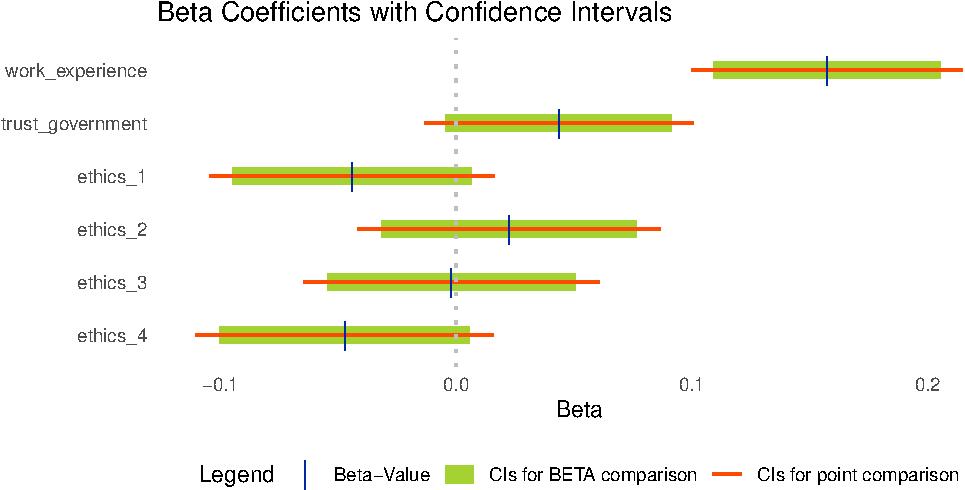
\includegraphics[width=0.85\textwidth,height=\textheight]{testthat_files/figure-pdf/unnamed-chunk-4-1.pdf}
\end{center}

\subsection{Teiltabelle}\label{teiltabelle}

\subsection{Analyse der
Voraussetzungen}\label{analyse-der-voraussetzungen}

In Abbildung~\ref{fig-reslev} ist gut zu erkennen.

\begin{figure}[H]

\centering{

\centering{

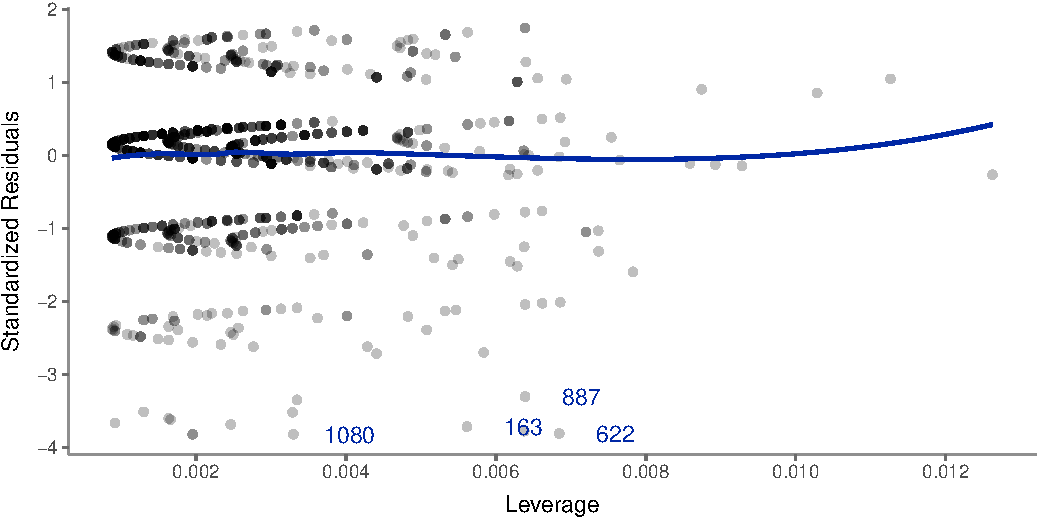
\includegraphics[width=0.85\textwidth,height=\textheight]{testthat_files/figure-pdf/fig-reslev-1.pdf}

}

\subcaption{\label{fig-reslev}}

}

\caption{\label{fig-reslev}residualsleverage plot}

\end{figure}%

Schaut man sich darüber hinaus Abbildung~\ref{fig-scaleloc} im schönen
UZH-Design an, wird einem alles klar.

\begin{figure}[H]

\centering{

\centering{

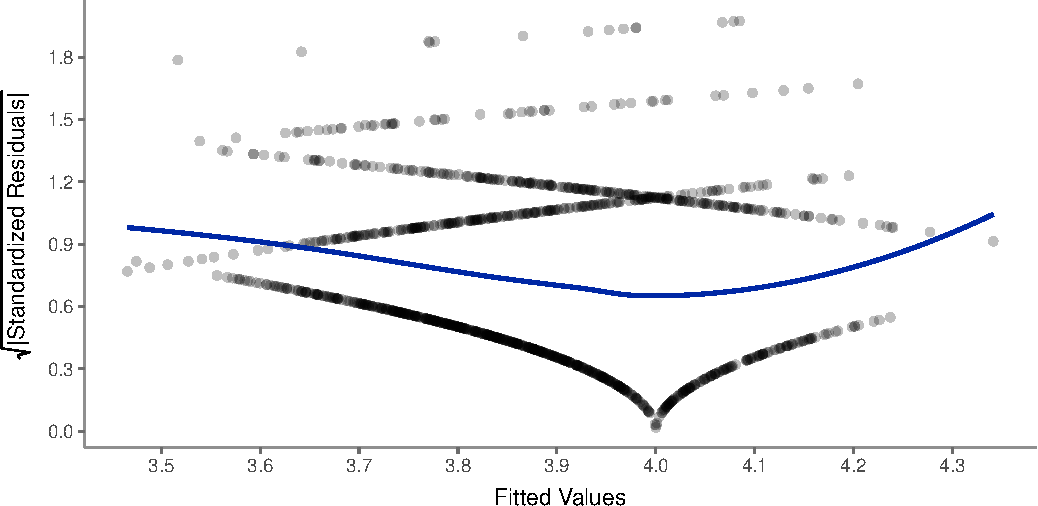
\includegraphics[width=0.85\textwidth,height=\textheight]{testthat_files/figure-pdf/fig-scaleloc-1.pdf}

}

\subcaption{\label{fig-scaleloc}}

}

\caption{\label{fig-scaleloc}scalelocation plot}

\end{figure}%

Nicht zuletzt sollte man sich die Residuen in Abhängigkeit der
geschätzten Werte ansehen, was im schönen Viridis-Design in
Abbildung~\ref{fig-resfit} durchaus möglich ist, auch wenn das dunkle
Lila nicht gut zu erkennen ist.

\begin{figure}[H]

\centering{

\centering{

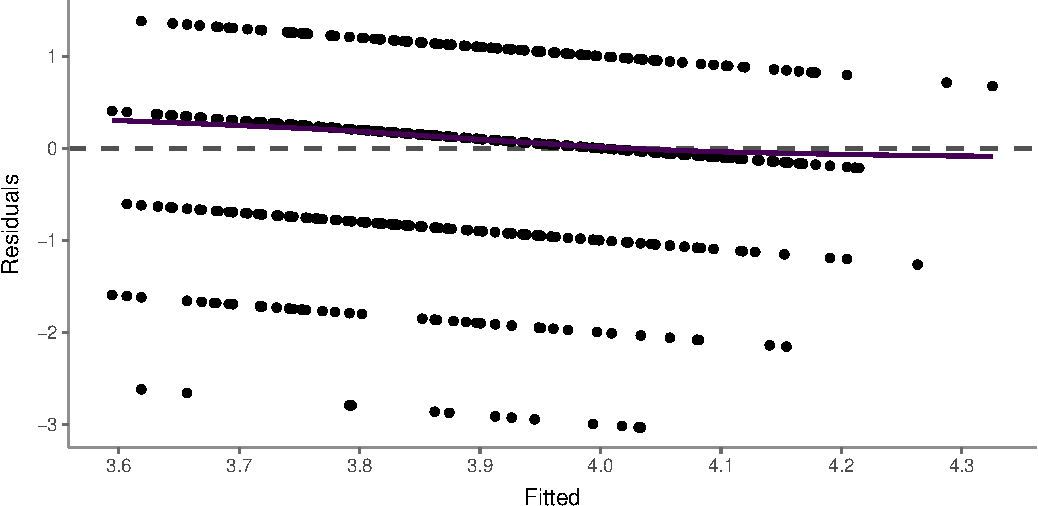
\includegraphics[width=0.85\textwidth,height=\textheight]{testthat_files/figure-pdf/fig-resfit-1.pdf}

}

\subcaption{\label{fig-resfit}}

}

\caption{\label{fig-resfit}residualsleverage plot}

\end{figure}%




\end{document}
